% This text is proprietary.
% It's a part of presentation made by myself.
% It may not used commercial.
% The noncommercial use such as private and study is free
% Sep. 2005 
% Author: Sascha Frank 
% University Freiburg 
% www.informatik.uni-freiburg.de/~frank/
%
% additional usepackage{beamerthemeshadow} is used
%  
%  \beamersetuncovermixins{\opaqueness<1>{25}}{\opaqueness<2->{15}}
%  with this the elements which were coming soon were only hinted
%\documentclass[8pt]{beamer}
\documentclass[10pt]{beamer}
\usepackage{etex}
\newenvironment<>{varblock}[2][\textwidth]{%
  \setlength{\textwidth}{#1}
  \begin{actionenv}#3%
    \def\insertblocktitle{#2}%
    \par%
    \usebeamertemplate{block begin}}
  {\par%
    \usebeamertemplate{block end}%
  \end{actionenv}}
%\usepackage{hyperref}
%\usepackage{natbib}
%\usepackage{beamerthemeshadow}
\usepackage{beamerinnerthemecircles, beamerouterthemeshadow}

\usepackage{amsmath,amssymb,amsfonts}
\usepackage[pdf]{pstricks}
%\usepackage{bbm}
%\usepackage{booktabs}
\usepackage{amsthm}
\usepackage{booktabs}
\usepackage{graphicx}
\usepackage{epsfig}
%\usepackage{graphics}

% MQ: This is to be able to compile on the Riksbank computer. Uncomment with my laptop. Ugly solution but will have to do for now.
%\usepackage{epstopdf}
%\epstopdfsetup{outdir=./}

\usepackage{rotating}

\usepackage{url}
%\usepackage{breqn}
%\usepackage{hyperref}
\usepackage[authoryear]{natbib}
\usepackage{setspace}
\usepackage{multirow}
%\usepackage{harvard}
\usepackage{xcolor}
%\usepackage{multicolumn}
\usepackage{algpseudocode}
\usepackage{sidecap}
\usepackage{bbm} 
\usepackage{courier}
\usepackage{tikz}
\usetikzlibrary{arrows,shapes,snakes,automata,backgrounds,petri}

\tikzset{
  treenode/.style = {align=center, inner sep=0pt, text centered,
    font=\sffamily},
  arn_n/.style = {treenode, circle, white, font=\sffamily\bfseries, draw=black,
    fill=black, text width=1.5em},% arbre rouge noir, noeud noir
  arn_r/.style = {treenode, circle, red, draw=red, 
    text width=1.5em, very thick},% arbre rouge noir, noeud rouge
  arn_x/.style = {treenode, rectangle, draw=black,
    minimum width=0.5em, minimum height=0.5em}% arbre rouge noir, nil
}
\beamertemplatenavigationsymbolsempty

\newenvironment{myenumerate}{\begin{enumerate}[(1)]}{\end{enumerate}} 
\sidecaptionvpos{figure}{c}
% FOR COLORING PARTS  OF TABLE
%\usepackage[beamer,customcolors]{hf-tikz}

%\tikzset{hl/.style={
%    set fill color=red!80!black!40,
%    set border color=red!80!black,
%  },
%}

\mode<presentation> {
    \usetheme{Madrid} %Frankfurt} %Bergen, Berkely, Berlin, Boadilla, CambridgeUS, Darmstadt,
                          %Frankfurt, Goettingen, Singapore, Warsaw
    \usecolortheme{beaver} %seahorse} %default} %beetle, seahorse, wolverine, dolphin, beaver
    %\useoutertheme[subsection=true]{smoothbars} 
    \usefonttheme{default}
    %\usecolortheme{red}
    

	\setbeamercolor{block title}{use=unstructure, fg=white, bg=purple!75!black} %{use=structure,fg=white,bg=purple!75!black}
	%\setbeamercolor{block body}{use=structure,fg=black,bg=white!20!white}    
    %\setbeamercolor{block body}{bg=white}
    \setbeamertemplate{enumerate items}[default]
    \setbeamercolor{enumerate item}{fg=purple!75!black} 
    \setbeamercolor{enumerate subitem}{fg=purple!75!black} 	 
	\setbeamercolor{itemize item}{fg=purple!75!black}  
	\setbeamertemplate{itemize item}[triangle]  
	\setbeamercolor{itemize subitem}{fg=purple!75!black}
	\setbeamertemplate{itemize subitem}[triangle]
	\setbeamertemplate{blocks}[framed]


}



%\usepackage{colortbl}
%\definecolor{yellow}{cmyk}{0,0.18,0.90,0.00}

%\usepackage{xcolor}

%\usepackage[authoryear]{natbib}
\begin{document}
\title[Lecture 2]{Bayesian Learning 732A46: Lecture 2}  
\author[Matias Quiroz]{Matias Quiroz\inst{1}$^{,}$\inst{2}}
\setbeamerfont{institute}{size=\fontsize{7pt}{8pt}}
\institute[LiU and Riksbank]{
  \inst{1}%
   Division of Statistics and Machine Learning, Link\"{o}ping University\\~\\
  \inst{2}%
   Research Division, Sveriges Riksbank\\
     
}

%\institute[Riksbank and LiU]{Sveriges Riksbank and Division of Statistics and Machine Learning, Link\"{o}ping University}

\date[]{March 2016} %\today 

%\usebackgroundtemplate{%
%  \vbox to \paperheight{\vfil\hbox to \paperwidth{\hfil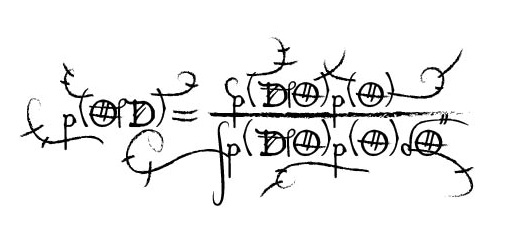
\includegraphics[width=1.5in]{Bayes.jpg}\hfil}\vfil}
%}

{
%\usebackgroundtemplate{\begin{center}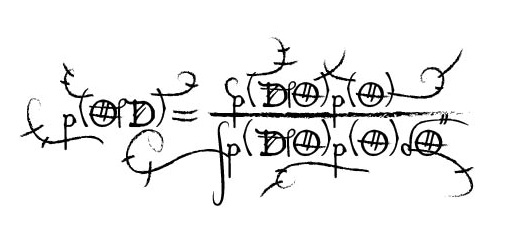
\includegraphics[width=0.4\paperwidth]{Bayes.jpg}\end{center}}
\usebackgroundtemplate{%
  \vbox to \paperheight{\hbox to \paperwidth{\hfil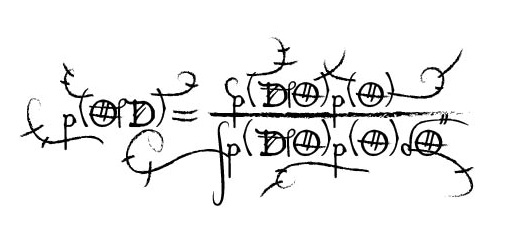
\includegraphics[width=2in]{Bayes.jpg}\hfil}}
}
\begin{frame}
\titlepage
\end{frame}
}
%\frame{\titlepage} 

%\frame{\frametitle{Overview of the talk}\tableofcontents}


\begin{frame}
\frametitle{Lecture overview}
\begin{itemize}
\item The Poisson model \bigskip{}

\item Conjugate priors \bigskip{}

\item Prior elicitation \bigskip{}

\item Non-informative priors
\end{itemize}	
\end{frame}

\begin{frame}
\frametitle{The Poisson model with a Gamma prior}
\begin{itemize}
\item \textbf{Model}: 
\[
y_{1},...,y_{n}\vert\theta\overset{iid}{\sim} \mathrm{Poisson}(y_i |\theta)=\frac{1}{y_i!}\theta^{y_i}\exp(-\theta), \quad \theta > 0.
\]
\item \textbf{Likelihood}
\[
p(y|\theta)=\prod\nolimits _{i=1}^{n}p(y_{i}|\theta)\propto\theta^{\sum\nolimits _{i=1}^{n}y_{i}}\exp(-\theta n),
\]
\item \textbf{Prior}
\[
p(\theta)\propto\theta^{\alpha_0-1}\exp(-\theta\beta_0)\propto \mathrm{Gamma}(\theta|\alpha_0,\beta_0)
\]
\textbf{\color{blue}Interpretation:} contains the info: $\alpha_0-1$ counts in $\beta_0$ observations.
\item \textbf{Posterior}
\small{
\begin{eqnarray*}
p(\theta|y) & \propto & \left[\prod\nolimits _{i=1}^{n}p(y_{i}|\theta)\right]p(\theta)\\
 & \propto & \theta^{\sum\nolimits _{i=1}^{n}y_{i}}\exp(-\theta n)\theta^{\alpha_0-1}\exp(-\theta\beta_0)\\
 & = & \theta^{(\alpha_0+\sum\nolimits _{i=1}^{n}y_{i})-1}\exp[-\theta(\beta_0+n)] \propto \mathrm{Gamma}(\theta|\underbrace{\alpha_0+\sum\nolimits _{i=1}^{n}y_{i}}_{\alpha_n},\underbrace{\beta_0+n}_{\beta_n}).
\end{eqnarray*}
}
\end{itemize}

\end{frame}


\begin{frame}{Poisson example - Bomb hits in London}


\[
n=576\text{, }\sum\nolimits _{i=1}^{n}y_{i}=229\cdot0+211\cdot1+93\cdot2+35\cdot3+7*4+1\cdot5=537.
\]
\textbf{Average number of hits} per region=$\bar{y}=537/576\approx0.9323.$
\[
p(\theta|y)\propto\theta^{\alpha_0+537-1}\exp[-\theta(\beta_0+576)]
\]
\[
E(\theta|y)=\frac{\alpha_0+\sum\nolimits _{i=1}^{n}y_{i}}{\beta_0+n}\approx\bar{y} \approx 0.9323,
\]
and
\[
SD(\theta|y)=\left(\frac{\alpha_0+\sum\nolimits _{i=1}^{n}y_{i}}{(\beta_0+n)^{2}}\right)^{1/2}=\frac{(\alpha_0+\sum\nolimits _{i=1}^{n}y_{i})^{1/2}}{(\beta_0+n)}\approx\frac{(537)^{1/2}}{576} \approx 0.0402.
\]
 if $\alpha_0$ and $\beta_0$ \textbf{are small compared} to $\sum\nolimits _{i=1}^{n}y_{i}$
and $n$.

\end{frame}


\begin{frame}{Poisson bomb hits in London}


\begin{figure}[h]
\centering
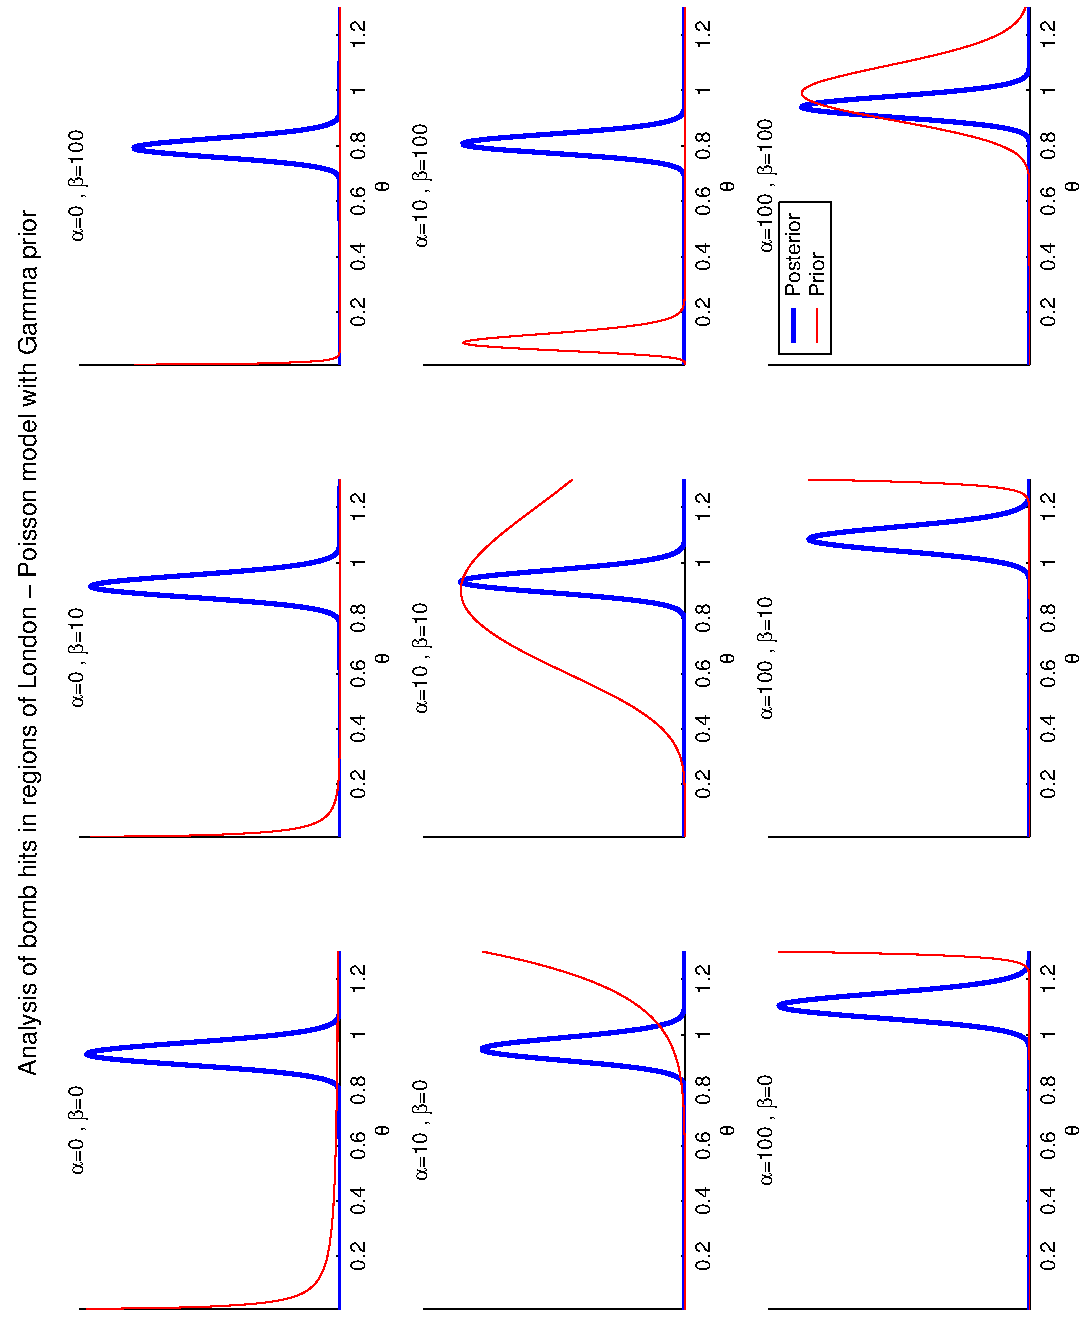
\includegraphics[width=0.65\columnwidth, angle=270]{BombHitsPoisson.pdf}
\end{figure}

\end{frame}


\begin{frame}{Poisson example - posterior intervals}

\begin{itemize}
\item \textbf{\textcolor{blue}{Bayesian 95\% interval}}: the probability
that the \textbf{unknown parameter} $\theta$ lies in the interval is 0.95.
\textbf{\color{red}What an easy and logical interpretation}! 
\item \textit{Approximate} $95\%$ \textbf{\textcolor{blue}{credible interval}} for
$\theta$ (for small $\alpha_0$ and $\beta_0$): 
\[
E(\theta|y)\pm1.96\cdot SD(\theta|y)=[0.8535;1.0111]
\]
\textbf{Assumes that} $p(\theta | y)$ is (approximately) normal.
\item An exact 95\% \textbf{\color{blue}equal-tail interval} is $[0.8550$; $1.0125]$ (assuming
$\alpha_0=\beta_0=0$)
\item \textbf{\textcolor{blue}{Highest Posterior Density}} (\textbf{\textcolor{blue}{HPD}})
interval contains the $\theta$ values with highest pdf. Here $[0.8525$; $1.0144]$, assuming $\alpha=\beta=0$.
\end{itemize}
\end{frame}

\begin{frame}{Illustration of different interval types}


\begin{center}
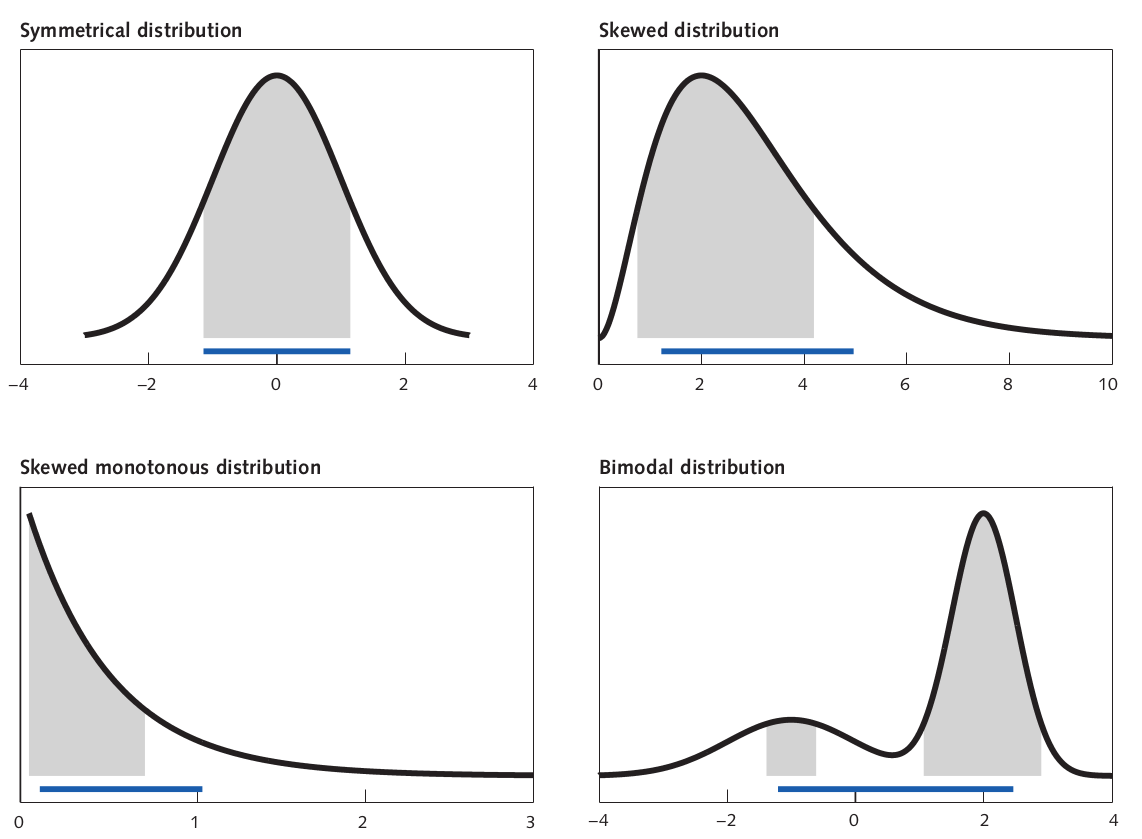
\includegraphics[scale=0.25]{IntervalTypes}
\par\end{center}

\end{frame}


\begin{frame}{{\Large{}Conjugate priors}}
\begin{itemize}
\item \textbf{Models} we have seen
\vspace{2mm}
\begin{center}
\begin{tabular}{llcl}
\textbf{\color{blue}Model} & $\textbf{\color{blue}Prior} \quad\quad\quad$ &  $\rightarrow$ & $\quad\quad\textbf{\color{blue}Posterior}$ \\
\vspace{2mm}
$\mathrm{Bernoulli}$ & $\theta \sim \mathrm{Beta}(\alpha_0, \beta_0)$ & $\rightarrow$ & $\theta | y \sim \mathrm{Beta}(\alpha_n, \beta_n)$ \\
\vspace{2mm}
$\mathrm{Normal}~(\sigma^2 \text{ known})$ & $\theta \sim \mathcal{N}(\mu_0, \tau_0^2)$ & $\rightarrow$ & $\theta | y \sim \mathcal{N}(\mu_n, \tau_n^2)$ \\

\vspace{2mm}$\mathrm{Poisson}$ & $\theta \sim \mathrm{Gamma}(\alpha_0, \beta_0)$ & $\rightarrow$ & $\theta | y \sim \mathrm{Gamma}(\alpha_n, \beta_n)$


\end{tabular}

\end{center}
\item \textbf{\textcolor{blue}{Conjugate priors}}: A prior is conjugate
to a model (likelihood) if the prior and posterior belong to the same
distributional family.
\item \textbf{\textcolor{blue}{Formally}}: Let $\mathcal{F}$ $=\{p(y|\theta),\theta\in\Theta\}$
be a class of sampling distributions. A family of distributions $\mathcal{P}$
is conjugate for $\mathcal{F}$ if 
\[
p(\theta)\in\mathcal{P\Rightarrow}\text{ }p(\theta|y)\in\mathcal{P}
\]
holds for all $p(y|\theta)\in\mathcal{F}$.
\item A Conjugate prior is \textbf{computationally convenient}.
\end{itemize}
\end{frame}

\begin{frame}{Prior elicitation}

\begin{itemize}
\item The prior should (ideally) be elicited by an \textbf{expert} ($\neq$ statistician, often)
\item Elicit the prior on a \textbf{quantity that she knows well} (maybe
log odds $\log\frac{\theta}{1-\theta}$ when the model is $\mathrm{Bern}(\theta)$).
\item The statistician can compute the \textbf{implied prior} on $\theta$ by transformation of variables.
\\ \textbf{\color{blue}Recall}: Let $p_u(u)$ be continuous and let $v=h(u)$ be a one-to-one transform.
$$p_v(v)=p_u(h^{-1}(v))|J|, \quad |J|=\text{determinant of } h^{-1}(v) \left[1\mathrm{-dim:}~\frac{d}{dv}h^{-1}(v)\right].$$

\item \textbf{Example}: expert believes $\phi = \log\frac{\theta}{1-\theta} \sim \mathcal{N}(0, 20)$. The implied prior on $\theta$ is [$u=\phi$, $v=\theta$, $h^{-1}(v) = \log  \frac{v}{1-v}$] $$p_{\theta}(\theta) =\mathcal{N}\left(\log\frac{\theta}{1-\theta}\Big|0, 20\right) \frac{1}{\theta (1-\theta)},\quad 0<\theta<1. $$

\item The example works out a \textbf{full distribution}.
\end{itemize}
\end{frame}



\begin{frame}{Prior elicitation, cont.}

\begin{itemize}
\item Working out \textbf{hyper-parameters from expert information}.
\item Elicit the prior by asking the expert simple questions: What is $E(\theta)$? or $V(\theta)$? 
\item The hyper-parameters are "backed out". \textbf{\color{blue}Example:} The prior is $$p(\theta)=\mathrm{Gamma}(\theta|\alpha_0, \beta_0), \quad \text{expert believes} \quad E(\theta)=2 \text{ and } V(\theta)=0.25.$$
$$E(\theta)=\frac{\alpha_0}{\beta_0}, \quad V(\theta)=\frac{\alpha_0}{\beta_0^2} \implies p(\theta)=\mathrm{Gamma}(\theta|16, 8).$$
\item \textbf{Show the expert some consequences} of her elicitated prior.
%\item \textbf{Beware of psychological effects}, such as anchoring.
\end{itemize}
\end{frame}



\begin{frame}{Prior elicitation - AR(p) example}

\begin{itemize}
\item \textbf{\color{blue}Autoregressive process} of order $p$
\begin{eqnarray*}
y_{t} & = & \mu + \phi_{1}\cdot(y_{t-1}-\mu)+...+\phi_{p}\cdot(y_{t-p}-\mu)+\varepsilon_{t},\text{ \ensuremath{\varepsilon_{t}\overset{iid}{\sim}N(0,\sigma^{2})}}
\end{eqnarray*}

\item \textbf{\color{blue}Informative prior} on the unconditional mean: $\mu\sim N(\mu_{0},\tau_{0}^{2})$.
\item \textbf{"Non-informative"}  prior on $\sigma^{2}$: $$p(\sigma^{2})\propto1/\sigma^{2} \quad [\text{uniform in the parameterization } p(\log(\sigma^2))\propto c]$$
\item \textbf{Assume} for simplicity that all $\phi_{i},\text{}i=1,...,p$ are independent
a priori, and $\phi_{i}\sim N(\mu_{i},\psi^2_{i})$.
\item Prior on $\phi=(\phi_{1},...,\phi_{p})$ centered on a persistent AR(1)
process: $$\mu_{1}=0.8,\text{}\mu_{2}=...=\mu_{p}=0.$$
\item \textbf{Prior variance} $\psi^2_{i}$ of the $\phi_{i}$ decay towards zeros: $Var(\phi_{i})=\frac{c}{i^{\lambda}}$,
so that ``longer'' lags are \textbf{more concentrated around zero} (less likely a priori). \item $\lambda$
is a parameter that can be used to determine the rate of decay. \textbf{Shrinkage/regularization/smoothness} prior.
\end{itemize}
\end{frame}

\begin{frame}{Different types of prior information}

\begin{itemize}
\item Real \textbf{\textcolor{blue}{expert information}}. Combo of previous
studies and experience.\medskip{}

\item Vague prior information, or even \textbf{\textcolor{blue}{non-informative
priors}}. \textbf{\color{red}Beware of improper priors - make sure the posterior is proper!}\medskip{}

\item \textbf{\textcolor{blue}{Smoothness priors}}. Regularization. Shrinkage.
Big thing in modern statistics/machine learning.\medskip{}

\item \textbf{\textcolor{blue}{Hierarchical priors}}. Model the uncertainty in the hyper-parameters. \textbf{Bayesian estimation of hyper-parameters}.


\end{itemize}
\end{frame}

\begin{frame}{{\Large{}Non-informative priors}}

\begin{itemize}
\item \textbf{Do not exist}! The "flatness" depends on the parametrization of the model.
\item Can be improper but still lead to a \textbf{proper posterior}.
\item \textbf{\color{blue}Reference prior}: A prior that plays a "minimal role". "Let the data speak for themselves".
\item Jeffreys' \textbf{\color{blue}invariance principle}: The prior should contain the same information \textbf{regardless of the parametrization} of the model.
\item \textbf{Jeffreys'} prior (1-dim)

\[
p(\theta) \propto \left|I(\theta)\right|^{1/2}, \quad I(\theta)=-E_{y}\left(\frac{d^2}{d\theta^2} \log p(y|\theta)\right),
\]
where $I(\theta)$ is the \textbf{\color{red}Fisher information} for $\theta$. 
\item The expectation\textbf{ is w.r.t data}... an \textbf{\color{blue}unconditional} (frequentist) feature! 
\item ... consequently, Jeffreys' prior \textbf{does not respect} the likelihood principle.
\item Can give \textbf{dubious results} in multivariate (parameter) models.
\end{itemize}
\end{frame}


\begin{frame}{Jeffreys' prior for Bernoulli trial data}
Let $y=(y_{1},...,y_{n})$
\[
y_{1},...,y_{n}|\theta\overset{iid}{\sim}\mathrm{Bern}(\theta)\quad\text{and}\quad \log p(y|\theta)=s\log\theta+f\log(1-\theta).
\]
\begin{eqnarray*}
\frac{d\log p(y|\theta)}{d\theta} & = &\frac{s}{\theta}-\frac{f}{(1-\theta)} \\
\frac{d^{2}\log p(y|\theta)}{d\theta^{2}} & = & -\frac{s}{\theta^{2}}-\frac{f}{(1-\theta)^{2}} \\ 
I(\theta) & = & \frac{E_{y}(s)}{\theta^{2}}+\frac{E_{y|\theta}(f)}{(1-\theta)^{2}} \\
~ & = & \frac{n\theta}{\theta^{2}}+\frac{n(1-\theta)}{(1-\theta)^{2}} = \frac{n}{\theta(1-\theta)}
\end{eqnarray*}
Thus, \textbf{the Jeffreys' prior} is
\[
p(\theta)=\left|I(\theta)\right|^{1/2} \propto \theta^{-1/2}(1-\theta)^{-1/2} \propto \mathrm{Beta}(\theta|1/2,1/2).
\]

\end{frame}


\begin{frame}{{\Large{}Non-informative priors - my two cents}}

\begin{itemize}
\item \textbf{Overrated}. Likelihood \textbf{dominates the prior} as more data becomes available.\bigskip{}
\item \textbf{\color{blue}State-of-the-art} models are \textbf{\color{red}very complex} these days. \textbf{Regularization/shrinkage/smoothness priors} to avoid over-fitting.\bigskip{}
\item Non-informative priors \textbf{\color{red}do not shrink}.
$$\textbf{Non-informative prior} \implies \textbf{no shrinkage} \implies \textbf{\color{red}no fun}.$$
\end{itemize}
\end{frame}

\end{document}

